%author: Man Cao, Lilong Jiang
\documentclass{article}
\usepackage[letterpaper]{geometry}
\usepackage[utf8]{inputenc}
\usepackage[T1]{fontenc}
%\usepackage{amsmath}
\usepackage{hyperref}
\usepackage{relsize}
\usepackage{graphicx}

\newcommand{\code}[1]{\textsf{\smaller\verb~#1~}}

\begin{document}

\title{CSE5243 Assignment 1}
\author{Man Cao(cao.235), Lilong Jiang(jiang.573)}
\maketitle

\section{Work Separation}
Lilong mainly worked on using the NLTK toolkit to compute the term--frequency
vector.
Man mainly worked on computing the tf--idf vector. In fact there were a lot of
overlapping during the work, we exchanged various ideas and wrote the this
report together.

\section{Parsing the file}
Since every file contains more than one piece of REUTERS news, it is not
a standard XML file. When we read the file, we add the
\code{<REUTERSList>} tag at the beginning of the file and
\code{</REUTERSList>} tag at the end of file to make it a standard XML
file.

We use Beautiful Soup (\url{http://www.crummy.com/software/BeautifulSoup/}) to
parse the XML structure. For every router news, we only extract the NEWID,
TOPICS, PLACES, TITLE and BODY contents.

\section{Determine the vocabulary of terms}
NLTK(\url{http://nltk.org/}) is used to determine the vocabulary of terms in the
TITLE and BODY contents.

\subsection{Tokenization}
We first tokenize the text into sentences. For every sentence, we then
chop it up into tokens.

\subsection{POS Tagging}
We tag each token in a sentence with part-of-speech information, and only keep
tokens which are nouns, verbs, adjectives or adverbs.
Since the POS tags in the treebank are different from the tags in the WordNet,
we map the POS tags in the treebank to the tags in the WordNet when we perform
the lemmatization.

\subsection{Normalization}
We normalize the tokens into lowercase and throw away the stop words,
punctuations, numbers and tokens whose length is 1.

\subsection{Lemmatization}
We lemmatize the tokens with WordNet. We noticed that the tokens need to be
in lowercase for the lemmatizer to work properly.

\subsection{Merging synonyms}
For the tokens which are synonyms, we replace them with the same token. We use
the SYNSET function of WordNet to find the synonyms.


\section{Constructing the feature vectors}
We construct two feature vectors: the term--frequency vector and tf--idf vector.
We use the class labels as provided in the TOPICS tags of each article.
\begin{itemize}
  \item The term--frequency vector \\
  For every term(token) in the document, we calculate the number of times it
  occurs in a document. We don't store the tokens that occur only once in the
  document.
  \item The tf--idf vector \\
  tf–-idf is the product of two statistics, term--frequency and inverse document
  frequency.
  Considering that sometime, the term--frequency is so large that it has a
  dominant impact on the final value, we use the augmented frequency, which is
  shown below:
  \begin{equation}
  \mathit{tf}(t,d) = 0.5 + \frac{0.5 \times f(t,d)}{\max\{f(w,d):w \in
  d\}}
  \end{equation}
  where $f(t,d)$ is the frequency of term $t$ in document $d$.
  The inverse document frequency is obtained by dividing the total number of
  documents by the number of documents containing the term, and then taking the
  logarithm of that quotient.
  \begin{equation}
  idf(t, D) = \log\frac{|D|}{|\{d \in D: t \in d\}|}  
  \end{equation}
  where $D$ is the total number of documents in the corpus.
\end{itemize}

\section{Output Format}
The two output files (feature vectors and tf--idf vectors) have the same format:
\begin{verbatim}
NEWID:<value> TOPICS:<value1, value2, ...> PLACES:<value1, value2, ...>
{<term1>:<value1>, <term1>:<value2>, ...}
\end{verbatim}
\noindent
Note that each document corresponds to two lines: the first line contains the
metadata of the document, the second line is the frequency/tf--idf vector.

\section{Implementation Details}
\begin{enumerate}
  \item  Since the text in the TITLE is much more important than the text in the
  BODY, we assign a higher weight for the tokens in the TITLE text.
  The weight is proportional to the length of all tokens in the document.
\begin{equation}
titleWeight = int(len(tokens) * 0.05 + 1)
\end{equation}
By ceiling the title weight, we can ensure the tokens exist even when the body
text is empty while having little impact on other documents.
  \item  For the news without topics, we assign 'None' to the class label.
  \item  For the news with multiple topics, we assign multiple topics to the
  class label, each topic separated by a semicolon.
  \item  In order to reduce the length of vector and avoid unnecessary
  computation, we only include the terms with high frequency. The
  frequency threshold is 1.
  \item  We have tried two popular stemming algorithms inside NLTK: Porter
  Stemmer and Snowball English Stemmer. However, the generated result is not as good as just
using the WordNet Lemmatizer with POS tags. For example, the word ``company'' is
stemmed into ``compani'', and the word ``venture'' is stemmed into ``ventur''. We
believe that a non-dictionary-based stemming algorithm does not provide
sufficiently accurate result in general. As a result, we decide not to use any
of those stemming algorithms at all.

\end{enumerate}

\section{Future Work}
Currently our preprocessor provides good result, but it runs quite
slow. It usually takes 1-5 seconds to process a single article, depending on
its length. More optimization could be done to improve the performance. An
obvious optimization is to support multithreading.

Other possible improvements on refining the extracted terms include spelling
correction, detecting named entities (which may be more important than regular
tokens), and handling abbreviations.

% \begin{figure}
% \centering
% 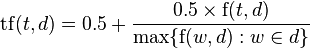
\includegraphics[width=0.5\textwidth]{formula1}
% \caption{test figure}
% \label{Fig:perf}
% \end{figure}
\end{document}

